\documentclass[11pt,letterpaper]{article}
\usepackage[lmargin=1in,rmargin=1in,tmargin=1in,bmargin=1in]{geometry}
\usepackage{../style/homework}
\usepackage{../style/commands}
\setbool{quotetype}{true} % True: Side; False: Under
\setbool{hideans}{false} % Student: True; Instructor: False

% -------------------
% Content
% -------------------
\begin{document}

\homework{14: Due 12/06}{Nature is written in mathematical language.}{Galileo Galilei}

% Problem 1
\problem{10} Sketch the function $f(x)= 7 - (x - 5)^2$.
	\[
	\fbox{
	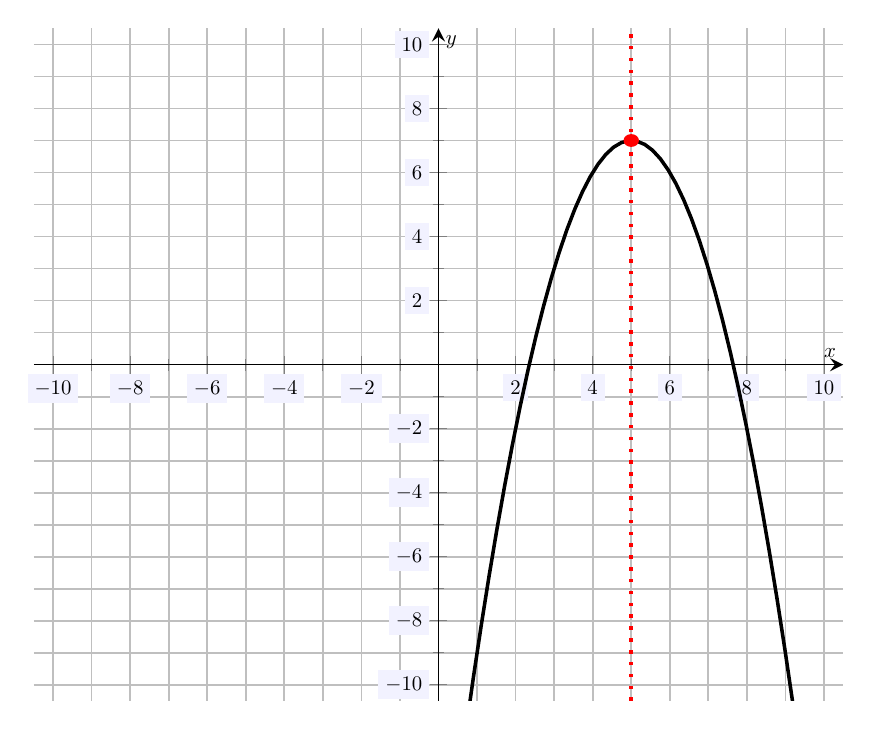
\begin{tikzpicture}[scale=1.5,every node/.style={scale=0.5}]
	\begin{axis}[
	grid=both,
	axis lines=middle,
	ticklabel style={fill=blue!5!white},
	xmin= -10.5, xmax=10.5,
	ymin= -10.5, ymax=10.5,
	xtick={-10,-8,-6,-4,-2,0,2,4,6,8,10},
	ytick={-10,-8,-6,-4,-2,0,2,4,6,8,10},
	minor tick = {-10,-9,...,10},
	xlabel=\(x\),ylabel=\(y\),
	]
	\addplot[line width=0.03cm,domain=-10:10,samples=100] ({x},{7 - (x - 5)^2});
	\draw[line width=0.03cm,red,dotted] (5,-10.5) -- (5,10.5);
	\draw[draw=none,fill=red] (5,7) circle (0.2);
	\end{axis}
	\end{tikzpicture}
	}
	\] \pspace

\sol Recall the vertex form of a quadratic function is $f(x)= a(x - P)^2 + Q$, where $(P, Q)$ is the vertex of the quadratic function and $a$ is the coefficient of $x^2$ from $f(x)= ax^2 + bx + c$. Observe that $f(x)= 7 - (x - 5)^2= -1(x - 5)^2 + 7$. Therefore, $a= -1 < 0$ and $(P, Q)= (5, 7)$. Therefore, the vertex is $(5, 7)$ and the parabola opens downwards because $a= -1 < 0$. The axis of symmetry is $x= 5$. Therefore, the plot should be symmetric about this line. This gives the sketch given above. 



\newpage



% Problem 2
\problem{10} Find the equation of the quadratic function shown below. Be sure to fully justify why your answer is correct.
	\[
	\fbox{
	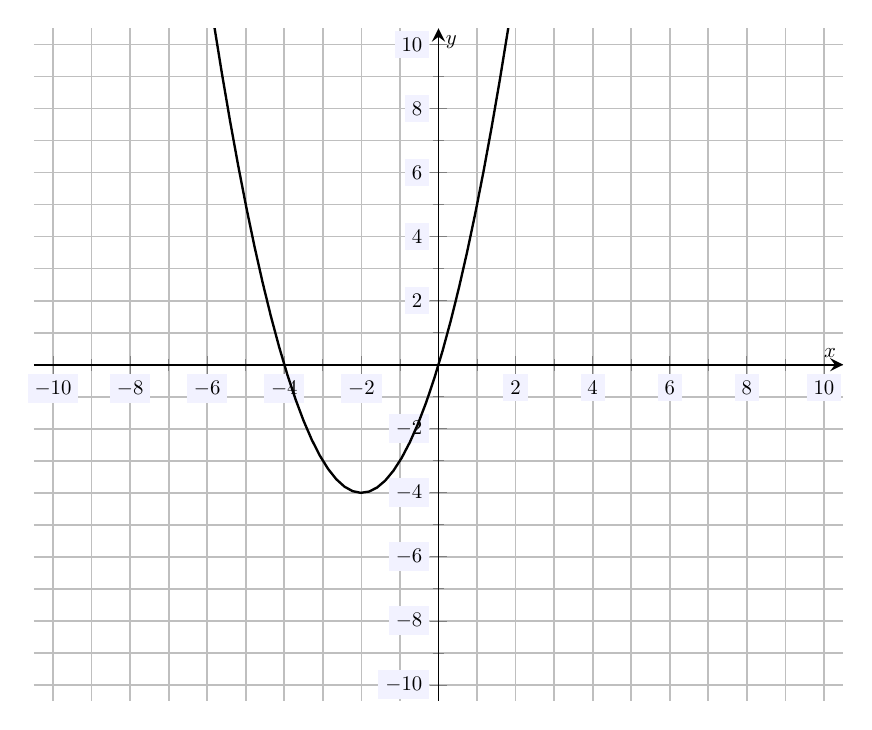
\begin{tikzpicture}[scale=1.5,every node/.style={scale=0.5}]
	\begin{axis}[
	grid=both,
	axis lines=middle,
	ticklabel style={fill=blue!5!white},
	xmin= -10.5, xmax=10.5,
	ymin= -10.5, ymax=10.5,
	xtick={-10,-8,-6,-4,-2,0,2,4,6,8,10},
	ytick={-10,-8,-6,-4,-2,0,2,4,6,8,10},
	minor tick = {-10,-9,...,10},
	xlabel=\(x\),ylabel=\(y\),
	]
	\addplot[line width= 0.02cm,samples=100,domain= -10.5:10.5] ({x},{(x + 2)^2 - 4});
	\end{axis}
	\end{tikzpicture}
	}
	\] \pspace

\sol We see that the quadratic function has zeros $x= -4$ and $x= 0$. We know that every quadratic function can be written in the form $f(x)= a(x - r_0)(x - r_1)$. But then $f(x)= a \big(x - (-4) \big)(x - 0)= a(x+ 4)x= ax(x + 4)$. We see also that the point $(-2, -4)$ is on the graph of $f(x)$. But then $f(-2)= -4$. Therefore, 
	\[
	\begin{gathered}
	f(x)= ax(x + 4) \\
	f(-2)= a \cdot -2 \cdot (-2 + 4) \\
	-4= -2a \cdot 2 \\
	-4= -4a \\
	a= 1
	\end{gathered}
	\]
Therefore, $f(x)= x(x + 4)= x^2 + 4x$. \pvspace{0.3cm}

\begin{center} OR \end{center} \pvspace{0.3cm}

We know the vertex form of a quadratic function is $f(x)= a(x - P)^2 + Q$, where $(P, Q)$ is the vertex. We can see from the graph of $f(x)$ that $(P, Q)= (-2, -4)$. Then $f(x)= a \big(x - (-2) \big)^2 + (-4)= a (x + 2)^2 - 4$. We can see also that $(0, 0)$ is on the graph of $f(x)$, i.e. $f(0)= 0$. But then\dots
	\[
	\begin{gathered}
	f(x)= a(x + 2)^2 - 4 \\
	f(0)= a (0 + 2)^2 - 4 \\
	0= a \cdot 2^2 - 4 \\
	4a= 4 \\
	a= 1
	\end{gathered}
	\]
Therefore, $f(x)= (x + 2)^2 - 4= (x^2 + 4x + 4) - 4= x^2 + 4x= x(x + 4)$. 



\newpage



% Problem 3
\problem{10} Consider the quadratic function $f(x)= x^2 - 6x + 14$.
	\begin{enumerate}[(a)]
	\item Find $a, b, c$ for this quadratic function.
	\item Does $f(x)$ open upwards or downwards? Explain.
	\item Is this quadratic function convex or concave? Explain. 
	\item Find the minimum value of $f(x)$, if it exists. If it does not exist, explain why.  
	\item Find the maximum value of $f(x)$, if it exists. If it does not exist, explain why. 
	\end{enumerate} \pspace

\sol 
\begin{enumerate}[(a)]
\item A quadratic function has the form $ax^2 + bx + c$. But then we can see that for $f(x)$, $a= 1$, $b= -6$, and $c= 14$. \pspace

\item Because $a= 1 > 0$, this quadratic function opens upwards. \pspace

\item Because $a= 1 > 0$, this quadratic function is convex. \pspace

\item Because $a= 1 > 0$, this quadratic function has a minimum value. We know the minimum value occurs at the vertex. So we need to find the vertex of $f(x)$. By completing the square, we have\dots
	\[
	\begin{gathered}
	x^2 - 6x + 14 \\
	x^2 - 6x + \left( \dfrac{-6}{2} \right)^2 - \left( \dfrac{-6}{2} \right)^2 + 14 \\
	x^2 - 6x + 9 - 9 + 14 \\
	(x^2 - 6x + 9) + (-9) + 14 \\
	(x - 3)^2 + 5
	\end{gathered}
	\]
Therefore, the vertex is $(3, 5)$. But then the minimum value for $f(x)$ is 5 and occurs when $x= 3$. \pspace

Alternatively, using the `evaluation method', we know the vertex occurs when $x= -\frac{b}{2a}= -\frac{-6}{2(1)}= \frac{6}{2}= 3$. But then the $y$-coordinate of the vertex $f(3)= 3^2 - 6(3) + 14= 9 - 18 + 14= 5$. Therefore, the vertex is $(3, 5)$ and the minimum output of $f(x)$ is 5. \pspace

\item Because $a= 1 > 0$, this quadratic function has no minimum value---the outputs of $f(x)$ get arbitrarily large. 
\end{enumerate}



\newpage



% Problem 4
\problem{10} Consider the quadratic function $f(x)= 4 - 2(x - 2)^2$.
	\begin{enumerate}[(a)]
	\item Find $a, b, c$ for this quadratic function.
	\item Does $f(x)$ open upwards or downwards? Explain.
	\item Is this quadratic function convex or concave? Explain. 
	\item Find the minimum value of $f(x)$, if it exists. If it does not exist, explain why.  
	\item Find the maximum value of $f(x)$, if it exists. If it does not exist, explain why. 
	\end{enumerate} \pspace

\sol 
\begin{enumerate}[(a)]
\item A quadratic function has the form $ax^2 + bx + c$. We expand $f(x)$: 
	\[
	f(x)= 4 - 2(x - 2)^2= 4 - 2(x^2 - 4x + 4)= 4 - 2x^2 + 8x - 8= -2x^2 + 8x - 4
	\]
But then we can see that for $f(x)$, $a= -2$, $b= 8$, and $c= -4$. \pspace

\item Because $a= -2 < 0$, this quadratic function opens downwards. \pspace

\item Because $a= -2 < 0$, this quadratic function is concave. \pspace

\item Because $a= -2 < 0$, this quadratic function has a maximum value. We know the maximum value occurs at the vertex. So we need to find the vertex of $f(x)$. But $f(x)$ was given in vertex form: $f(x)= 4 - 2(x - 2)^2= -2(x - 2)^2 + 4$. Therefore, the vertex is $(2, 4)$. Then the maximum value for $f(x)$ is 4 and occurs when $x= 2$. 

\item Because $a= -2 < 0$, this quadratic function has no minimum value---the outputs of $f(x)$ get arbitrarily small. 
\end{enumerate}


\end{document}